\documentclass[border=2pt]{standalone}
\usepackage{amsmath}
\usepackage{tikz}
\usetikzlibrary{calc,shapes.arrows}
\begin{document}
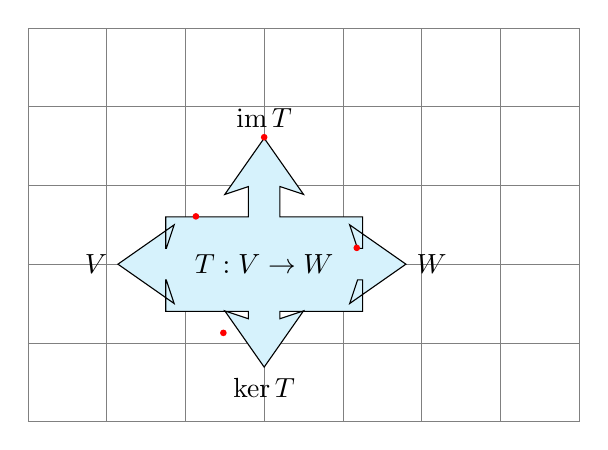
\begin{tikzpicture}
  \draw[help lines] (-3,-2) grid (4,3);
  \node[arrow box,draw,fill=cyan!16,minimum width=25mm,minimum height=12mm,
    arrow box arrows={north:16mm from center,south:7mm,east:18mm from center,west:6mm},
    arrow box shaft width=4mm,arrow box head extend=3mm,
    arrow box head indent=1mm,arrow box tip angle=70] (map) at (0,0) {$T:V\to W$};
  \fill[red] (map.north arrow tip) circle (1.2pt)
    (map.before east arrow head) circle (1.2pt)
    (map.after south arrow tip) circle (1.2pt)
    (map.145) circle (1.2pt);
  \node[above] at (map.north arrow tip) {$\operatorname{im}T$};
  \node[right] at (map.east arrow tip) {$W$};
  \node[left] at (map.west arrow tip) {$V$};
  \node[below] at (map.south arrow tip) {$\ker T$};
\end{tikzpicture}
\end{document}
